\zerar
\chapter{Resultados e Discussão}
\label{cap:resultados}

Em nosso estudo utilizamos os pacotes de otimização GLPK (GNU Linear Programming Kit) e Cplex da
IBM. Os resultados finais, entretanto, são baseados apenas na utilização da ferramenta Cplex, uma
vez que a mesma provou ser mais eficiente. Além disso, o otimizador Cplex pôde ser utilizado
diretamente a partir de nosso código, alimentando o modelo gerado através da API Java fornecida pela
IBM. Por outro lado, como o GLPK não fornece API apropriada, sua utilização se limitou a geração do
modelo em arquivo (formato mps) e posterior execução do otimizador em um processo separado, sendo
necessário realizar um {\it parsing} no arquivo de saída gerado para obtenção dos resultados.

Implementamos os métodos de solução do PDV descritos no Capítulo~\ref{cap:heuristicas}. Os 
parâmetros utilizados, que garantem a legalidade das viagens geradas, são apresentados na
Tabela~\ref{tab:parametros} e baseiam-se na legislação brasileira para aviação comercial regular.

Todos os testes foram realizados em um computador utilizando um processador Intel Core~i3 64~bits, 
com 4~Gb de memória RAM, rodando o sistema operacional MacOS~10.6. Toda a implementação foi escrita 
em Java (JDK~1.6.33).

\begin{table}
	\begin{center}
		\begin{tabular}{|l|l|l|}
			\hline 
			\bf Parâmetro & \bf Descrição & \bf Valor \\
			\hline \hline 
			\verb|MAX_LEGS| & Máximo de pernas por jornada & 5 \\ \hline
			\verb|MAX_TRACKS| & Máximo de trocas de aeronave por jornada & 2 \\ \hline
			\verb|MAX_FLIGHT_TIME| & Total máximo de voo por jornada & 9,5 h \\ \hline
			\verb|MAX_DUTY_TIME| & Duração máxima de uma jornada & 11,5 h \\ \hline
			\verb|MIN_SIT_TIME| & Tempo mínimo de conexão & 30 min \\ \hline
			\verb|MAX_SIT_TIME| & Tempo máximo de conexão & 120 min \\ \hline
			\verb|BRIEFING_TIME| & Tempo para o {\it briefing} & 0 min \\ \hline
			\verb|DEBRIEFING_TIME| & Tempo para o {\it debriefing} & 0 min \\ \hline
			\verb|MIN_REST_TIME| & Tempo mínimo de repouso & 12 h \\ \hline
			\verb|MAX_REST_TIME| & Tempo máximo de repouso & 36 h \\ \hline
			\verb|MAX_DUTIES| & Máximo de jornadas por viagem & 2, 3 ou 4 \\ \hline
			\end{tabular} 
			\caption{Parâmetros utilizados na geração das viagens.}
			\label{tab:parametros}
	\end{center}
\end{table}

%%%%%%%%%%%%%%%%%%%%%%%%%%%%%%%%%%%%%%%%%%%%%%%%%%%%%%%%%%%%%%%%%%%%%%%%%%%%%%%%%%%%%%%%%%%%%%%%%%%%

\section{Análise Preliminar}
\label{sec:preliminar}

O objetivo desta análise preliminar foi definir o limite de utilização do procedimento de geração
de viagens e do otimizador na resolução exata do modelo {\it set partition} (\ref{eq:sppv}).
Com essa finalidade, construímos alguns gráficos que relacionam o tempo de geração e otimiazação 
utilizado em nossa implementação, em função do número de etapas da entrada do problema.

Para estudar a influência do número de pernas isoladamente, restringimos a entrada apenas para um
conjunto de voos entre duas localidades, São Paulo (CGH) e Rio de Janeiro (SDU), considerando os
trechos diárias oferecidos na ponte-aérea pela companhia aérea Gol. Um total de 62 pernas 
(31 de CGH para SDU e 31 de SDU para CGH) representam a instância global de entrada.

Vale observar que o caso da ponte-aérea é um pouco atípico no sentido de que representa um malha 
muito densa de voos: muitas etapas são oferecidas de ida e volta num curto intervalo de tempo, 
criando muitas conexões legais (arcos) entre os nós da rede de voos gerada. Com isso, o número
de viagens dado pela procedimento de busca no grafo explode rapidamente.

O gráfico da Figura~\ref{fig:pairings} mostra o número de viagens geradas em função do número de
etapas na ponte-aérea. As viagens foram geradas para a base CGH. São apresentadas três curvas, uma
para cada valor do parâmetro \verb|MAX_DUTIES| (2, 3 e 4). Observe a escala logarítmica do eixo
vertical. O comportamento praticamente linear das curvas indica um crescimento exponencial do número
de viagens que podem ser geradas. Observe ainda que a taxa de crescimento é maior quanto maior o
número máximo de jornadas permitidas, já que nesse caso permite-se um número muito maior de
combinações. Para \verb|MAX_DUTIES| = 4, encontrou-se um número da ordem de $10^8$ viagens com
apenas 36 pernas.

\begin{figure}[htp]
	\begin{center}
		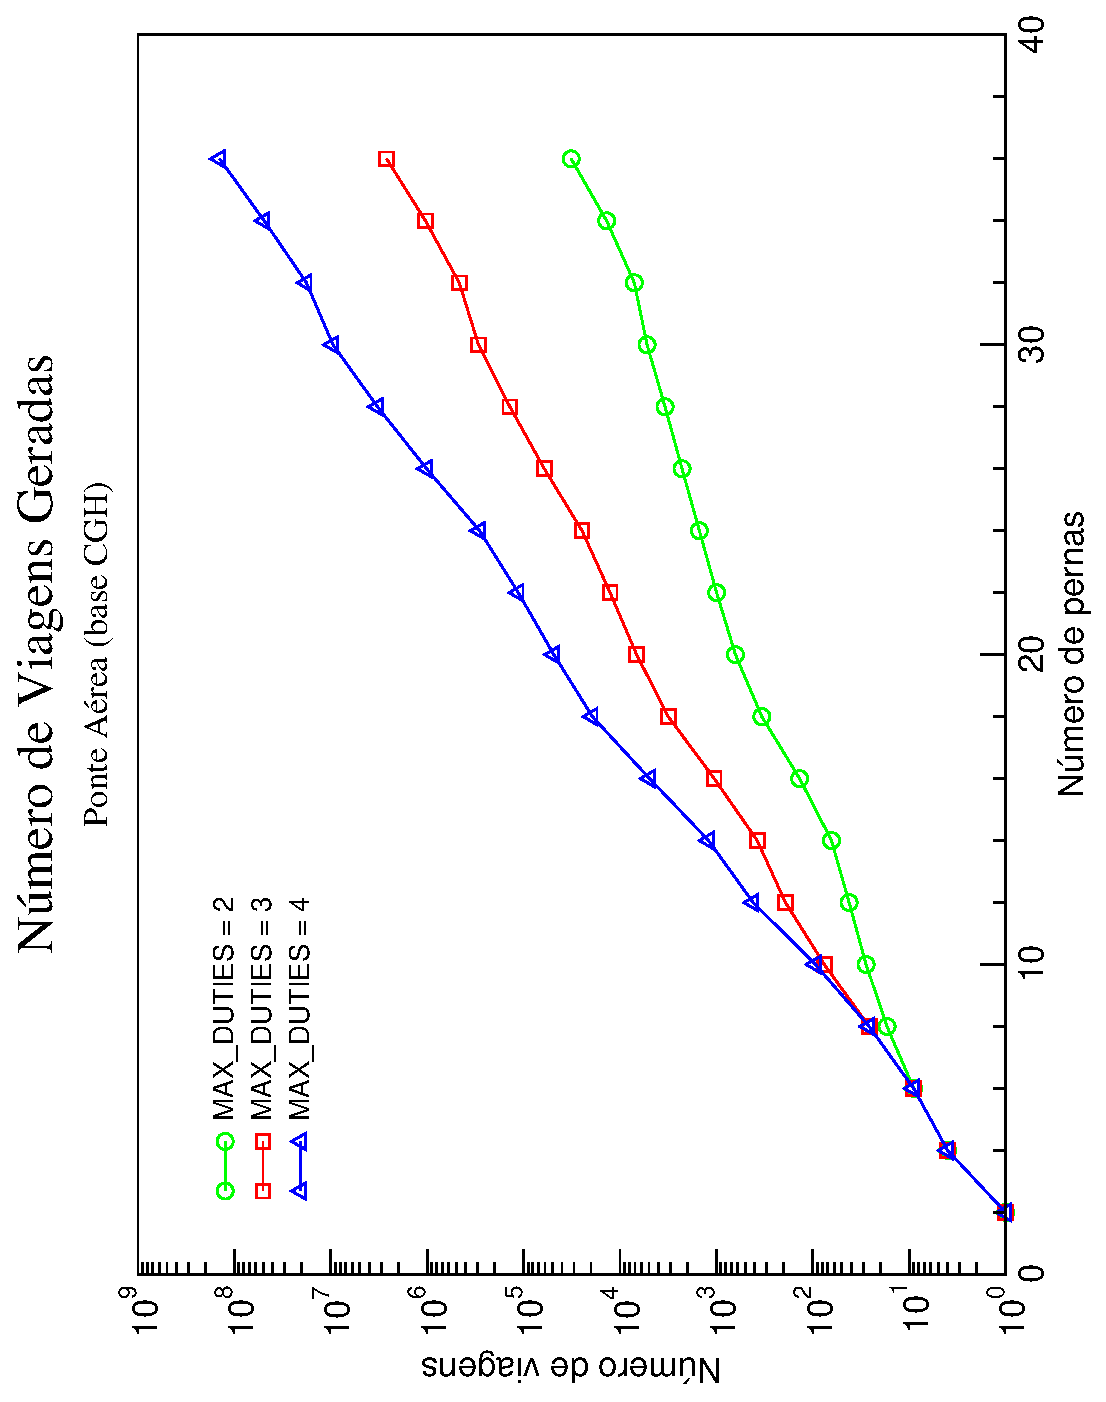
\includegraphics[scale=0.45,angle=-90]{fig/number_of_pairings.eps}
		\caption{Número de viagens geradas em função do número de pernas utilizadas na construção da
		rede de voos.}
		\label{fig:pairings}
	\end{center}
\end{figure}

O consumo de tempo gasto pelo algoritmo de busca em profundidade também foi medido em função do 
número de pernas. Os resultados são apresentados na Figura~\ref{fig:generation}. O comportamento das
curvas indicam também um crescimento exponencial do tempo gasto pelo algoritmo, ainda que ele seja
executado de forma rápida (para \verb|MAX_DUTIES| = 4, encontrou-se um tempos da ordem de $10^4$~ms 
para 36 pernas).

\begin{figure}[htb]
	\begin{center}
		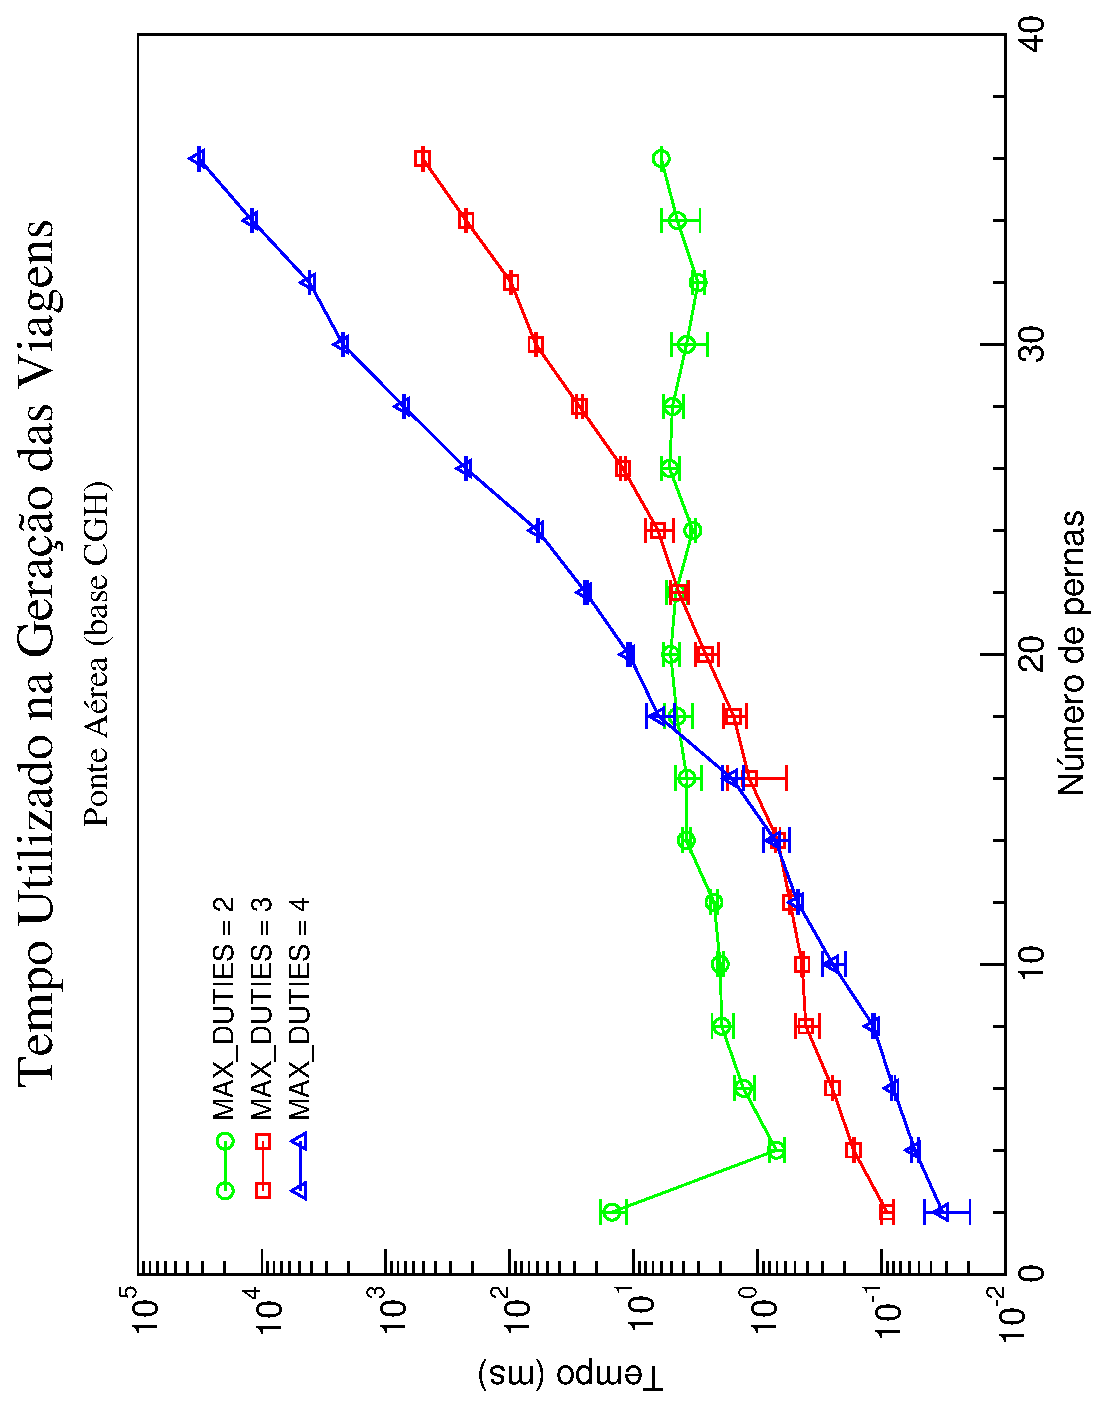
\includegraphics[scale=0.45,angle=-90]{fig/generation_time.eps}
		\caption{Tempo gasto na geração das viagens em função do número de pernas utilizadas na 
		construção da rede de voos. São apresentados valor médio $\pm$ desvio-padrão, considerando 5 
		medidas para cada ponto. O primeiro ponto da curva verde encontra-se um pouco fora,
		provavelmente devido a algum transiente da máquina, visto que ele foi o primeiro a
		ser processado.}
		\label{fig:generation}
	\end{center}
\end{figure}

O tempo gasto pelo otimizador GLPK para resolver o modelo proposto é apresentado no gráfico da 
Figura~\ref{fig:glpk}. Mais uma vez, observa-se um crescimento exponencial muito forte (note a 
escala logarítmica do eixo vertical) em função do número de etapas considerado. A 
Figura~\ref{fig:cplex} mostra os resultados obtidos para o otimizador Cplex. 

\begin{figure}[htb]
	\begin{center}
		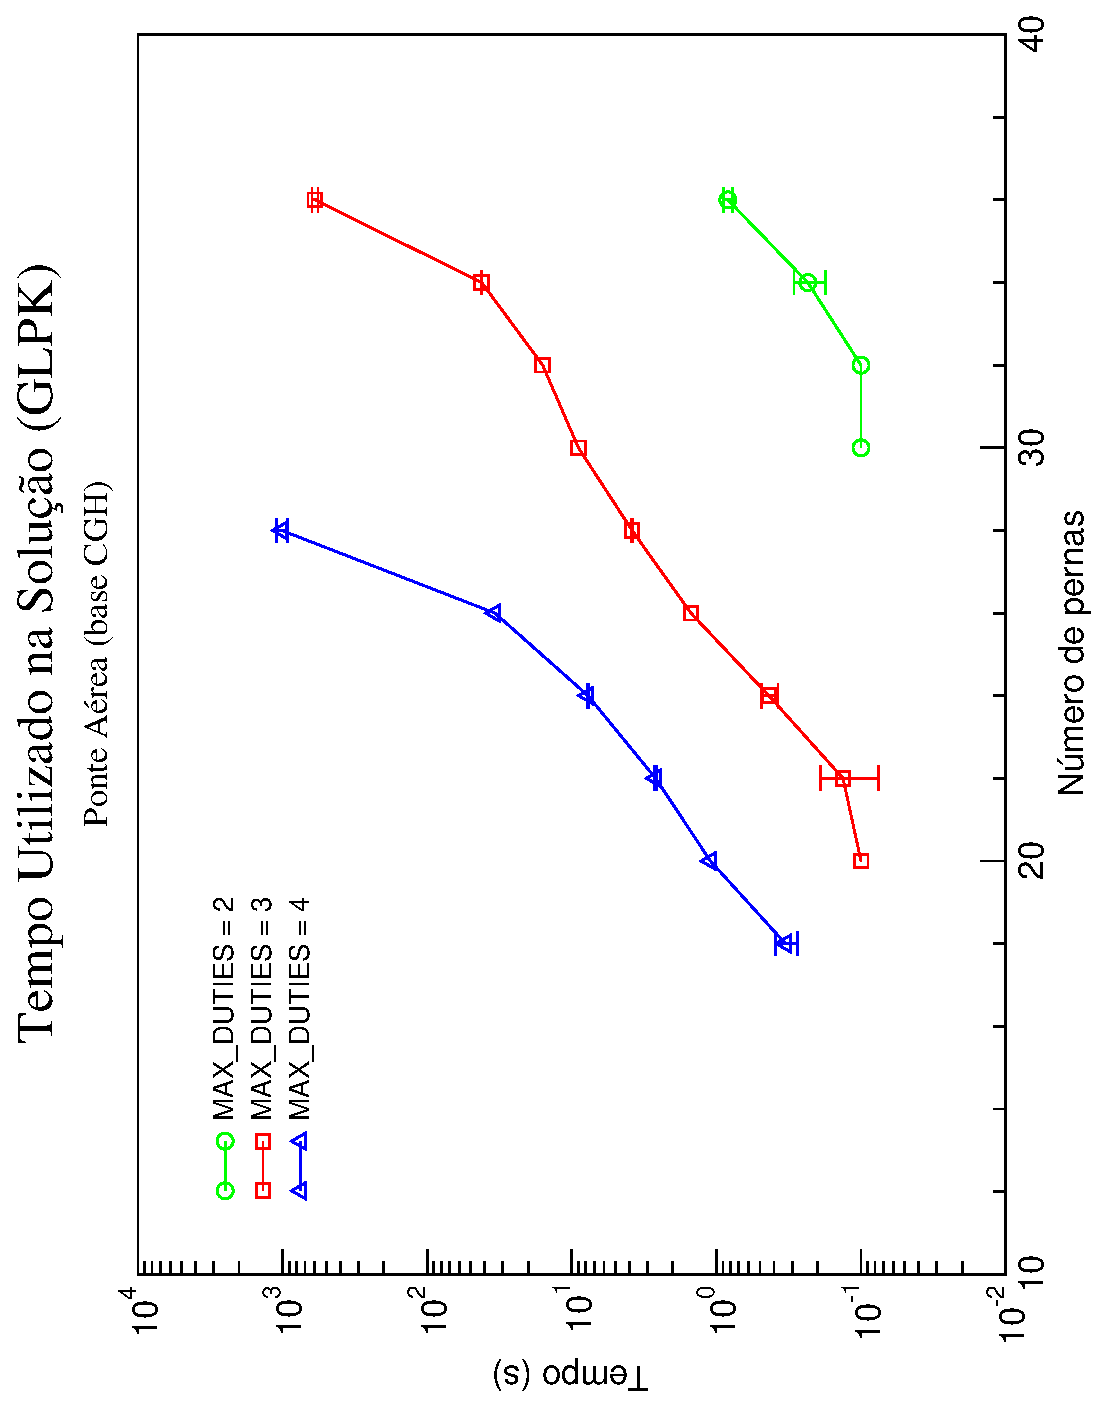
\includegraphics[scale=0.45,angle=-90]{fig/glpk_solution_time.eps}
		\caption{Tempo utilizado pelo otimizador GLPK na obtenção de uma solução inteira, em função do 
		número de etapas. São apresentados valor médio $\pm$ desvio-padrão, considerando 3 medidas para 
		cada ponto. Valores medidos com tempo de execução de 0,0~s não são apresentados (número pequeno 
		de pernas). Os últimos pontos da curva azul não puderam ser estimados, mesmo após algumas horas 
		de processamento.}
		\label{fig:glpk}
	\end{center}
\end{figure}

\begin{figure}[htb]
	\begin{center}
		\includegraphics[scale=0.45,angle=0]{fig/cplex_solution_time.eps}
		\caption{Resultados obtidos para o otimizador Cplex. Valem as mesmas observações feitas na 
		legenda da Figura~\ref{fig:glpk}.}
		\label{fig:cplex}
	\end{center}
\end{figure}

%%%%%%%%%%%%%%%%%%%%%%%%%%%%%%%%%%%%%%%%%%%%%%%%%%%%%%%%%%%%%%%%%%%%%%%%%%%%%%%%%%%%%%%%%%%%%%%%%%%%

\section{Instâncias}
\label{sec:instancias}

Os métodos heurísticos implementados foram testados em dados reais dados pelas instâncias listadas
na tabela~\ref{tab:instancias}. Os dados se referem a voos diários oferecidos no passado pelas
companhias Gol e WebJet. 

Na tabela são indicados o nome da instância, a companhia a qual pertence, a frota de aeronaves a que
se refere, o número de etapas e o número de trilhos. O trilho identifica o conjunto de etapas que
uma determinada aeronave da frota deve executar diariamente. No caso de uma frota com $k$ aeronaves,
deverão ser fornecidos $k$ trilhos distintos.

A instância PA\_62 se refere a voos na ponte-aérea estudados na análise preliminar. A instância mais
difícil se refere à 73G\_340, com 340 etapas diárias e 40 trilhos de aeronaves.

\begin{table}[htb]
	\begin{center} 
		\begin{tabular}{|l|l|l|l|l|}
			\hline 
			{\bf Instância} & {\bf Cia} & {\bf Frota} & {\bf Etapas} & {\bf Trilhos} \\ 
			\hline \hline
			73H\_26 & Gol & 737-800 & 26 & 5 \\ 
			738\_48 & WebJet & 737-800 & 48 & 7 \\ 
			733\_92 & WebJet & 737-300 & 92 & 12 \\
			73G\_340 & Gol & 737-700 & 340 & 40 \\
			PA\_62 & Gol & 737-800S & 62 & 6 \\ \hline
		\end{tabular}
		\caption{Caracterização das instâncias utilizadas para testes em nosso estudo.}
		\label{tab:instancias}
	\end{center}
\end{table}

%%%%%%%%%%%%%%%%%%%%%%%%%%%%%%%%%%%%%%%%%%%%%%%%%%%%%%%%%%%%%%%%%%%%%%%%%%%%%%%%%%%%%%%%%%%%%%%%%%%%

\section{Soluções Exatas}
\label{sec:solucoes_exatas}

Apenas três instâncias (pequenas) puderam ser resolvidas exatamente pela solução do modelo {\it set
partition} (\ref{eq:sppv}), com um tempo de processamento aceitável. A descrição dos problemas é
apresentada na Tabela~\ref{tab:problemas}.

\begin{table}[htb]
	\begin{center} 
		\begin{tabular}{|c|c|c|}
			\hline 
			{\bf Problema} & {\bf Instância} & {\bf Bases} \\ 
			\hline \hline
			P1 & 73H\_26 & GRU \\ 
			P2 & 738\_48 & GRU e GIG \\ 
			P3 & 733\_92 & GRU, GIG e POA \\ \hline
		\end{tabular}
		\caption{Caracterização dos problemas resolvidas exatamente através dos modelos 
		{\it set partition} e {\it set cover}. GRU = São Paulo, GIG = Rio de Janeiro e POA = Porto
    Alegre.}
		\label{tab:problemas}
	\end{center}
\end{table}

Na resolução dos problemas, foram utilizados os parâmetros da Tabela~\ref{tab:parametros}. Além
disso, limitou-se a 2 o número máximo de trocas de aeronaves por jornada. Com isso, forçamos a
tripulação acompanhar, na medida do possível, o trilho percorrido pela aeronave, reduzindo a
possibilidade de conexões em cada localidade. Naturalmente os tempos de conexão serão reduzidos,
tornando as viagens geradas mais baratas e diminuindo o número total de variáveis geradas. Além
disso, esse procedimento torna a solução mais robusta, uma vez que o atraso de uma aeronave não
acarretará atraso na saída de outro voo que dependa daquela aeronave na troca.

O custo de uma viagem foi calculado como sendo o tempo ``ocioso'' relativo no qual o tripulante está 
trabalhando mas não está voando, ou seja, pela diferença entre o tempo total de uma viagem, menos o 
tempo total de voo efetuado, descontando ainda os tempos mínimos regulamentares de conexão entre 
pernas e de descanso entre jornadas, dividido pelo tempo total de voo. Esse custo avalia de forma 
relativa a produtividade de uma viagem, o qual deve ser minimizado na solução final.

Os resultados obtidos são apresentados e resumidos na Tabela~\ref{tab:resultados}. Nela são 
indicadas a instância resolvida, o número total de variáveis geradas, o número de viagens na 
solução, o custo da solução e o tempo de processamento do otimizador (Cplex).

\begin{table}[htb]
	\begin{center} 
		\begin{tabular}{|c|c|c|c|c|}
			\hline 
			{\bf Problema} & {\bf Variáveis} & {\bf Viagens} & {\bf Custo} & {\bf Tempo (s)} \\ 
			\hline \hline
			P1 & 180 & 6 & 6,952 & $< 1$ \\ 
			P2 & 66411 & 6 & 6,436 & 3,75 \\
			P3 & 1023818 & 11 & 6,942 & 170,86 \\ \hline
		\end{tabular}
		\caption{Resultados obtidos na geração e otimização de viagens para os problemas consideradas.}
		\label{tab:resultados}
	\end{center}
\end{table}

As mesmas instâncias 73H\_26, 738\_48, 733\_92 também foram resolvidas utilizando o modelo {\it set
cover} (\ref{eq:scpdv}), o qual admite a existência de {\it deadheading}. Os resultados obtidos
foram idênticos aos listados na Tabela~\ref{tab:resultados}. Em particular, todas as variáveis
artificiais $y_i$ receberam valor zero na solução final, indicando a não necessidade de {\it
deadheading}.

%%%%%%%%%%%%%%%%%%%%%%%%%%%%%%%%%%%%%%%%%%%%%%%%%%%%%%%%%%%%%%%%%%%%%%%%%%%%%%%%%%%%%%%%%%%%%%%%%%%%

\section{Uma Solução Explícita}
\label{sec:solucao_explicita}

Para tornar mais concreto a entrada e a saída do problema, apresentamos na Tabela~\ref{tab:73H_26} o
conjunto de etapas referentes a instância 73H\_26\footnote{Não há problema de confidencialidade nos
dados apresentados, uma vez que os mesmos se referem a dados do passado liberados pela companhia
aérea.}. A mesma representa 26 trechos oferecidos diariamente pela companhia aérea Gol para uma
frota especial de 5 aeronaves B737-800. Para cada etapa são fornecidos o seu número, aeroporto de
origem, aeroporto de destino, horário local de decolagem (DEP) e horário local de pouso (ARR) e o
trilho correspondente.

Na Tabela~\ref{tab:pairings} listamos as 6 viagens geradas como solução do problema de otimização.
Cada etapa na tabela apresenta o número do voo, origem e destino, horário local de decolagem e 
pouso, e o trilho executado. O custo final resultante foi de 6,952, para um total de 180 variáveis 
geradas, considerando a base GRU (São Paulo). Observe a presença de uma viagem bate-volta (4),
bem como uma viagem de 3 dias de duração (5).

\begin{table}[htb]
	\begin{center}
		\scalebox{0.73}{
		\begin{tabular}{|cccccc|}
			\hline 
			{\bf Número} & {\bf Origem} & {\bf Destido} & {\bf DEP} & {\bf ARR} & {\bf Trilho} \\
			\hline \hline
			7625 & GRU &	GIG	 &  07:00	 &  08:00  & 1 \\
			7622 & GIG &	GRU	 &  09:00	 &  09:55	 & 1 \\
			7622 & GRU &	CCS	 &  11:00	 &  15:30	 & 1 \\
			7622 & CCS &	AUA	 &  16:10	 &  17:55	 & 1 \\
			7623 & AUA &	CCS	 &  21:20	 &  22:05	 & 1 \\
			7623 & CCS &	GRU	 &  22:45	 &  06:00	 & 1 \\
			1841 & CWB &	GRU	 &  07:52	 &  08:55	 & 2 \\
			1902 & GRU &	NAT	 &  11:00	 &  14:20	 & 2 \\
			1903 & NAT &	GRU	 &  15:30	 &  19:10	 & 2 \\
			1704 & GRU &	MAO	 &  21:15	 &  00:10	 & 2 \\
			1798 & GRU &	REC	 &  08:05	 &  11:21	 & 3 \\
			1149 & REC &	GRU	 &  12:04	 &  15:30	 & 3 \\
			7680 & GRU &	AEP	 &  18:25	 &  21:15	 & 3 \\
			7681 & AEP &	GRU	 &  22:40	 &  01:30	 & 3 \\
			1705 & MAO &	GRU	 &  03:42	 &  08:35	 & 4 \\
			1766 & GRU &	CWB	 &  09:20	 &  10:16	 & 4 \\
			1846 & CWB &	GRU	 &  11:13	 &  12:15	 & 4 \\
			7480 & GRU &	ASU	 &  13:05	 &  13:50	 & 4 \\
			1847 & GRU &	CWB	 &  18:10	 &  19:20	 & 4 \\
			1767 & CWB &	GRU	 &  20:56	 &  21:50	 & 4 \\
			1566 & GRU &	CWB	 &  22:35	 &  23:30	 & 4 \\
			7481 & ASU &	GRU	 &  14:30	 &  17:25	 & 4 \\
			7678 & GRU &	AEP	 &  08:00	 &  10:50	 & 5 \\
			7679 & AEP &	GRU	 &  11:50	 &  14:35	 & 5 \\
			7658 & GRU &	EZE	 &  15:15	 &  18:15	 & 5 \\
			7659 & EZE &	GRU	 &  20:35	 &  23:25	 & 5 \\ \hline
	\end{tabular}}
	\caption{Dados que caracterizam a instância 73H\_26.}
	\label{tab:73H_26}
	\end{center}
\end{table}


\begin{table}[htb]
	\begin{center}
		\scalebox{0.73}{
		\begin{tabular}{|c|c|ccccc|}
			\hline
			{\bf Viagem} & {\bf Jornada} & \multicolumn{5}{|c|}{\bf Etapa} \\ \hline \hline
			\multirow{6}{*}{1} & \multirow{4}{*}{1}  
			  & 7625 & GRU-GIG & 07:00 & 08:00 & 001 \\
			& & 7622 & GIG-GRU & 09:00 & 09:55 & 001 \\
			& & 7622 & GRU-CCS & 11:00 & 15:30 & 001 \\
			& & 7622 & CCS-AUA & 16:10 & 17:55 & 001 \\ \cline{2-7}
			                       & \multirow{2}{*}{2}
				& 7623 & AUA-CCS & 21:20 & 22:05 & 001 \\
			& &	7623 & CCS-GRU & 22:45 & 06:00 & 001 \\ \hline \hline
			\multirow{2}{*}{2} & \multirow{2}{*}{1}  		
				& 1902 & GRU-NAT & 11:00 & 14:20 & 002 \\
			& & 1903 & NAT-GRU & 15:30 & 19:10 & 002 \\ \hline \hline
			\multirow{2}{*}{3} & \multirow{1}{*}{1}  		
				& 1704 & GRU-MAO & 21:15 & 00:10 & 002 \\ \cline{2-7}
                           	& \multirow{1}{*}{2}
				&	1705 & MAO-GRU & 03:42 & 08:35 & 004 \\ \hline \hline
			\multirow{2}{*}{4} & \multirow{2}{*}{1}  		
				& 1798 & GRU-REC & 08:05 & 11:21 & 003 \\
			& & 1149 & REC-GRU & 12:04 & 15:30 & 003 \\ \hline \hline			
			\multirow{10}{*}{5} & \multirow{3}{*}{1}  
				&	1847 & GRU-CWB & 18:10 & 19:20 & 004 \\
			& &	1767 & CWB-GRU & 20:56 & 21:50 & 004 \\
			& &	1566 & GRU-CWB & 22:35 & 23:30 & 004 \\ \cline{2-7}
                           		& \multirow{4}{*}{2}
				&	1841 & CWB-GRU & 07:52 & 08:55 & 002 \\
			&	&	1766 & GRU-CWB & 09:20 & 10:16 & 004 \\
			&	&	1846 & CWB-GRU & 11:13 & 12:15 & 004 \\
			&	&	7480 & GRU-ASU & 13:05 & 13:50 & 004 \\ \cline{2-7}
                           		& \multirow{3}{*}{3}
				&	7481 & ASU-GRU & 14:30 & 17:25 & 004 \\
			&	&	7680 & GRU-AEP & 18:25 & 21:15 & 003 \\
			&	&	7681 & AEP-GRU & 22:40 & 01:30 & 003 \\ \hline \hline
			\multirow{4}{*}{6} & \multirow{3}{*}{1}  
				& 7678 & GRU-AEP & 08:00 & 10:50 & 005 \\
			& & 7679 & AEP-GRU & 11:50 & 14:35 & 005 \\
			&	& 7658 & GRU-EZE & 15:15 & 18:15 & 005 \\ \cline{2-7}
                           	 & \multirow{1}{*}{2}
				& 7659 & EZE-GRU & 20:35 & 23:25 & 005 \\ \hline
		\end{tabular}}
		\caption{Conjunto de viagens obtido como solução ótima da instância 73H\_26.}
		\label{tab:pairings}
	\end{center}
\end{table}

%%%%%%%%%%%%%%%%%%%%%%%%%%%%%%%%%%%%%%%%%%%%%%%%%%%%%%%%%%%%%%%%%%%%%%%%%%%%%%%%%%%%%%%%%%%%%%%%%%%%

\section{Aplicação das Heurísticas}
\label{sec:aplicacao_heuristicas}

Como esperado, os métodos exatos mostraram-se ineficientes para instâncias grandes ou até mesmo para
uma instância pequena de ponte-aérea. Apesar de não garantir solução ótima, os métodos aproximados
apresentaram soluções aceitáveis, em alguns casos ótimas, em tempos de execução pequenos. A seguir
apresentaremos os resultados específicos de cada método implementado.

Todos os testes forma realizados nas instâncias da Tabela~\ref{tab:instancias}, considerando apenas
a base GRU para geração de viagens. O número máximo de jornadas foi escolhido 4, menos no caso da
ponte-aérea (PA\_62), onde consideramos o valor 2 (no máximo um pernoite).

A função de custo utilizada para cada viagem foi uma que buscava maximizar a relação de horas de voo
por horas de jornada. Buscamos com isso viagens com jornadas produtivas para os tripulantes. Mais
especificamente, se $F_j$ é o tempo total de voo de uma viagem $j$ e $D_j$ o seu tempo total de
jornada, então $c_j = D_j / F_j$.

%%%%%%%%%%%%%%%%%%%%%%%%%%%%%%%%%%%%%%%%%%%%%%%%%%%%%%%%%%%%%%%%%%%%%%%%%%%%%%%%%%%%%%%%%%%%%%%%%%%%

\subsection{Tabela de Resultados}
\label{sec:valores}

A Tabela~\ref{tab:comparacao} mostra os resultados do processo de otimização para as três
heurísticas. São apresentados tempo de processamento em segundos (CPU) e valor da função objetivo
(OBJ) para a melhor solução encontrada. O valor de DH entre parênteses indica o número de etapas
sobrecobertas na solução ({\it deadheads}). A tabela ainda explora os resultados para três valores
dos parâmetros $k$ e $L$ dos métodos de busca local e algoritmo genético híbrido, respectivamente.

O método de geração de colunas fornece um limitante inferior para o custo da solução, já que resolve
de forma ótima a relaxação linear do problema. O custo obtido pelos demais métodos é expresso em
\% com relação ao valor desse limitante inferior.

\begin{table}[ht]
\begin{center}
\scalebox{0.72}{
\begin{tabular}{cc|c|c|c|c|c|c|c|c|c|c|}
	\cline{3-12}
	& &
	\multicolumn{2}{|c|}{\bf 73H\_26} & 
	\multicolumn{2}{|c|}{\bf 738\_48} & 
	\multicolumn{2}{|c|}{\bf 733\_92} & 
	\multicolumn{2}{|c|}{\bf 73G\_340} & 
	\multicolumn{2}{|c|}{\bf PA\_62} \\
	\cline{3-12}
	& & OBJ (DH) & CPU & OBJ (DH) & CPU & OBJ (DH) & CPU & OBJ (DH) & CPU & OBJ (DH) & CPU \\

	\hline
	\multicolumn{2}{|c|}{GC} & 
	5,696 (0)  & 0,26  & 
	6,230 (0) & 0,54  & 
	10,973 (0) & 1,36  & 
	42,744 (0) & 54,02 & 
	10,103 (0) & 1,13 \\

	\hline
	\multicolumn{1}{|c|}{\multirow{3}{*}{BL}} 
	& $k = 2$ & 
	0\% (0) & 1,10   & 
	$>$100\% (116) & 1,22   & 
  $>$100\% (124) & 3,16   & 
	$>$100\% (654) & 208,44 & 
	$>$100\% (8) & 0,79 \\
	\multicolumn{1}{|c|}{} 
	& $k = 3$ &
	0\% (0) & 1,48    & 
	14,1\% (0) & 7,91    & 
	8,1\% (0) & 18,68   & 
	32,5\% (9) & 1303,53 & 
	87,7\% (0) & 1,31 \\
	\multicolumn{1}{|c|}{} 
	& $k = 4$ & 
	0\% (0) & 1,81 & 
	0\% (0) & 11,46 & 
	7,7\% (0) & 99,09 & 
	25,5\% (11) & 2182,31 & 
	0\% (0)   & 17,83 \\

	\hline
	\multicolumn{1}{|c|}{\multirow{3}{*}{AG}} 
	& $L = 1$ & 
	0\% (0) & 1,39 & 
	78,1\% (2) & 4,35 & 
	$>$100\% (9) & 8,30 & 
	$>$100\% (476) & 1074,97 & 
	56,2\% (0) & 4,31 \\
	\multicolumn{1}{|c|}{} 
	& $L = 5$ & 
	0\% (0) & 4,17 & 
	13,8\% (0) & 13,19 & 
	46,4\% (0) & 10,79 & 
	$>$100\% (208) & 763,19 & 
	36,2\% (0) & 13,99 \\
	\multicolumn{1}{|c|}{} 
	& $L = 10$ & 
	0\% (0) & 11,01 & 
	0\% (0) & 33,99 & 
	72,2\% (3)3 & 17,85 & 
	$>$100\% (78) & 482,10 & 
	30,5\% (0) & 27,50 \\
	\hline
\end{tabular}}
\caption{Resultados do processo de otimização para as três heurísticas: GC = geração de colunas,
BL = busca local e AG = algoritmo genético.}
\label{tab:comparacao}
\end{center}
\end{table}

A partir dos dados da Tabela~\ref{tab:comparacao}, faremos uma análise dos resultados para cada uma 
das heurísticas estudadas nas seções seguintes.

%%%%%%%%%%%%%%%%%%%%%%%%%%%%%%%%%%%%%%%%%%%%%%%%%%%%%%%%%%%%%%%%%%%%%%%%%%%%%%%%%%%%%%%%%%%%%%%%%%%%

\subsection{Busca Local}
\label{sec:resultados_busca}

O método de Busca Local revelou-se eficiente para todos os tamanhos de instância, produzindo
soluções ótimas para instâncias pequenas e médias, e próximas ao ótimo para instâncias grandes. O
número de viagens, $k$, escolhido por iteração deve ser definido {\it a priori}. 

A Figura~\ref{fig:ls_results} mostra a evolução do processo de otimização para cada um dos problemas
considerados e cada valor de $k$ escolhido.

\begin{figure}[htbp]
	\begin{center}
		\includegraphics[scale=0.5]{fig/localsearch_results.eps}
		\caption{Evolução do processo de otimização para o método da busca local (custo $\times$ 
		iteração).}
		\label{fig:ls_results}
	\end{center}
\end{figure}

%%%%%%%%%%%%%%%%%%%%%%%%%%%%%%%%%%%%%%%%%%%%%%%%%%%%%%%%%%%%%%%%%%%%%%%%%%%%%%%%%%%%%%%%%%%%%%%%%%%%

\subsection{Algoritmo Genético}
\label{sec:resultados_genetico}

O algoritmo genético tradicional provou-se inviável para instâncias com muitos voos pois necessita
da geração de todos as viagens para gerar sua população e realizar mutações. Além disso as soluções
para problemas pequenos mostraram-se muito ruins, convergindo rapidamente para mínimos locais longe
do ótimo. Através da utilização de busca local para gerar indivíduos melhores, obtivemos sensíveis
ganhos em relação ao método original. Apesar disso as características apresentadas pelo método
híbrido não se modificaram. 

A Figura~\ref{fig:ga_results} mostra a evolução do processo de otimização para cada um dos problemas
considerados e cada valore de $L$ escolhido. Como pode ser visto no gráfico, algumas das soluções
obtidas não foram boas devido à dificuldade do método em remover {\it deadheads}. Lembramos que o
custo dos {\it deadheads} são altos, o que explica soluções ruins como em 737\_92 e 73G\_340.

\begin{figure}[htbp]
	\begin{center}
		\includegraphics[scale=0.5]{fig/genetic_results.eps}
		\caption{Evolução do processo de otimização para o algoritmo genético (custo médio da população
		$\times$ geração).}
		\label{fig:ga_results}
	\end{center}
\end{figure}

Assim como o algoritmo de busca local, as iterações são muito rápidas, mas é necessário um grande
número de iterações na busca por soluções aceitáveis. O algoritmo genético híbrido é um método que
converge rapidamente para um mínimo local e depende de um grande número de parâmetros. Uma sintonia
fina é necessária no ajuste dos parâmetros porém sua realização é demasiadamente difícil devido à
natureza aleatória do algoritmo.

%%%%%%%%%%%%%%%%%%%%%%%%%%%%%%%%%%%%%%%%%%%%%%%%%%%%%%%%%%%%%%%%%%%%%%%%%%%%%%%%%%%%%%%%%%%%%%%%%%%%

\subsection{Geração de Colunas}
\label{sec:resultados_cg}

O método de geração de colunas conseguiu obter soluções ótimas fracionárias para todas as instâncias
disponíveis, produzindo um conjunto reduzido de viagens, que contém tais soluções, em tempos muito
reduzidos. 

Estas soluções indicam um limitante inferior para o problema inteiro. O algoritmo
caracteriza-se por uma pequena quantidade de iterações, porém cada iteração é mais demorada do que
os métodos anteriores.

A Figura~\ref{fig:cg_results} mostra a evolução do processo de otimização para cada um dos problemas
considerados. Os gráficos nos mostram que a convergência ocorre rapidamente e em poucas
iterações obtemos a solução ótima. Por exemplo, na instância 73G\_340, foram necessárias apenas
50 iterações, consumindo um tempo total de processamento menor do que um minuto. 

\begin{figure}[htbp]
	\begin{center}
		\includegraphics[scale=0.5]{fig/cg_results.eps}
		\caption{Evolução do processo de otimização para o procedimento de geração de colunas (custo 
		$\times$ iteração). São apresentados os resultados para as cinco instâncias
		estudadas.}
		\label{fig:cg_results}
	\end{center}
\end{figure}

%%%%%%%%%%%%%%%%%%%%%%%%%%%%%%%%%%%%%%%%%%%%%%%%%%%%%%%%%%%%%%%%%%%%%%%%%%%%%%%%%%%%%%%%%%%%%%%%%%%%

\section{Desenvolvimento e Implementação}
\label{sec:implementacao}

O trabalho foi desenvolvido em Java pois é a linguagem orientada a objetos com a qual temos mais
experiência. A existência de uma API do Cplex para Java também foi importante para a nossa escolha.
Procuramos programar sempre em trio para que todos os integrantes do grupo tivessem conhecimento
total sobre o código e, quando isso não era possível, realizávamos programação pareada. Utilizamos
um repositório Git para termos controle de versões. A seguir descrevemos as etapas percorridas 
durante a elaboração do código.

\begin{enumerate}
\item {\bf Modelagem de Dados:}
Iniciamos o trabalho com a modelagem das entidades necessárias para representar os diversos
elementos do problema de geração de viagens. Implementamos uma rede de voos através de um grafo em
que nós representam voos e arestas suas conexões. Realizamos testes de unidade (JUnit) para garantir
a robustez da base do projeto.
\item {\bf Geração de Pairings:}
O primeiro passo foi gerar a rede de voos através da leitura de um arquivo texto contendo
informações sobre os voos. A seguir, implementamos as regras utilizadas pelas companhias aéreas do
Brasil para a geração de viagens legais. As viagens foram então geradas percorrendo-se a rede de
voos, buscando caminhos legais entre a fonte e o sorvedouro. Assim como na etapa anterior, diversos
testes de unidade foram implementados.
\item {\bf Modelagem do Problema:}
Nessa etapa foi necessário transformar as informações sobre voos e viagens em entradas para os
otimizadores Cplex e GLPK. Definimos a função objetivo que determina o custo de uma solução e o
modelo (\ref{eq:scpdv}) utilizando a API do Cplex. Para o cálculo do custo de uma viagem definimos 
uma interface que pode ser implementada por classes concretas para representar o custo desejado 
pelo cliente (veja Figura~\ref{fig:cost_interface}).
\item {\bf Análise Preliminar:}
Com todos os elementos necessários para gerar viagens e resolver problemas de forma exata,
realizamos testes para analisar as limitações computacionais do PDV. Os objetivos eram verificar a
quantidade total de viagens geradas e o tempo consumido tanto para gerar as viagens quanto para
resolver o problema.
\item {\bf Heurísticas:}
Após comprovar a ineficiência dos métodos exatos, iniciamos a implementação de meta-heurísticas.
\item {\bf Busca Local:}
Iniciamos essa fase implementando o algoritmo de busca local pois é amplamente utilizado em
problemas de otimização e faz uso do {\it set cover}, que foi desenvolvido na etapa anterior.
\item {\bf Algoritmo Genético Híbrido:}
O algoritmo genético tradicional implementado em um primeiro momento mostrou-se muito deficiente
quando comparado ao método de busca local. Sentimos que era necessário realizar mudanças e
desenvolvemos um método híbrido utilizando busca local na geração de indivíduos. Devido à grande
quantidade de parâmetros, realizamos testes com configurações distintas a fim de se observar as
mudanças de comportamento do método.
\item {\bf Geração de Colunas:}
Com a obtenção dos duais através da API do Cplex, a geração de colunas foi implementada através de
uma busca no grafo de voos utilizando os custos reduzidos. Como o método proporciona um limitante
inferior para o problema inteiro, adquiri-se informações importantes para uma melhor análise dos
resultados.
\end{enumerate}

\begin{figure}[htbp]
	\begin{center}
		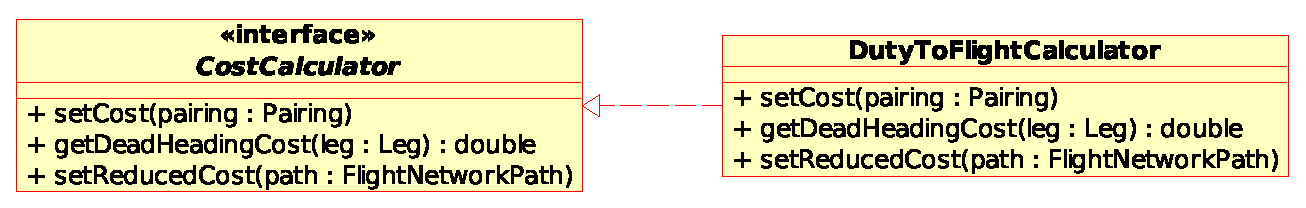
\includegraphics[scale=0.65]{fig/cost_calculator.eps}
		\caption{Interface {\it CostCalculator} e a sua relação com a implementação concreta
    DutyToFlightCalculator. Note que, com este acoplamento, diversas implementações para o cálculo
    do custo são possíveis.}
		\label{fig:cost_interface}
	\end{center}
\end{figure}


%%%%%%%%%%%%%%%%%%%%%%%%%%%%%%%%%%%%%%%%%%%%%%%%%%%%%%%%%%%%%%%%%%%%%%%%%%%%%%%%%%%%%%%%%%%%%%%%%%%%

\subsection{Algumas Métricas do Código}
\label{sec:metricas}

Através do {\it plugin} Metrics do Eclipse obtivemos algumas informações sobre o código: 

\begin{itemize}
\item 55\% de cobertura de testes. Os métodos heurísticos são difíceis de se testar e por isso a
cobertura total foi reduzida. No entanto, a base do código teve cerca de 80\% de cobertura e 
garantiu a robustez desejada;
\item 5600 linhas de código; 
\item 16 pacotes; 
\item 78 classes; 
\item 795 métodos;
\item Número médio de linhas por método = $3,639 \pm 3,198$;
\item Complexidade cyclomática média = $1,585 \pm 1,072$;
\item Número de parâmtros médio por método = $0,588 \pm 0,789$;
\item Profundidade de aninhamento de bloco médio = $1,115 \pm 0,452$;
\item LOCM ({\it lack os cohesion of methods}) médio = $0,263 \pm 0,328$;
\item Nível de abstratividade média = $0,097 \pm 0,148$.
\end{itemize}

%%%%%%%%%%%%%%%%%%%%%%%%%%%%%%%%%%%%%%%%%%%%%%%%%%%%%%%%%%%%%%%%%%%%%%%%%%%%%%%%%%%%%%%%%%%%%%%%%%%%